\subsection{Luthfi Muhammad Nabil/1174035}
\subsubsection{Pemahaman Teori}
\begin{enumerate}
	\item Fungsi adalah sintaks yang terdiri dari nama fungsi, parameter input variabel, dan variabel kembali. Pada python, nama fungsi diawali dengan def dan pada sintaks paling akhir (setelah parameter) adalah titik dua. Aturan penamaan dari fungsi sama dengan penamaan sebuah variabel yang salah satunya yaitu case sensitive. Untuk penulisan parameter tidak harus memasukan inputan dan batas untuk penulisan variabel pada parameter tidak memiliki batas atau bisa lebih dari satu dengan pemisah tanda koma. Nilai yang dapat dikembalikan oleh fungsi dapat berupa variabel yang mau dikembalikan. Berikut contoh dari koding fungsi : 
	\lstinputlisting[firstline=1, lastline=4]{src/chapter3/chap3_1174035_teori.py}
	\item Paket merupakan sebuah file yang berisikan fungsi - fungsi yang dapat dipakai. Untuk pemanggilan fungsi diperlukan keyword import untuk memanggil paket tersebut. berikut contoh pemakaian dari paket : 
	\lstinputlisting[firstline=6, lastline=8]{src/chapter3/chap3_1174035_teori.py}
	\item Class merupakan cetak biru dari sebuah objek yang dibuat. Objek merupakan instansi dari sebuah class. Atribut merupakan variabel atau yang menampung nilai pada sebuah objek. Fungsi adalah sebuah pembungkus kumpulan instruksi pada sebuah program. Berikut contohnya : 
	\lstinputlisting[firstline=10, lastline=24]{src/chapter3/chap3_1174035_teori.py}
	\item Pemanggilan sebuah kelas diawali dari sebuah paket dipanggil terlebih dahulu, lalu kelas akan disimpan ke variabel untuk diinisiasi sebagai objek. Berikut contoh pemanggilan dari kelas : 
	\lstinputlisting[firstline=26, lastline=29]{src/chapter3/chap3_1174035_teori.py}
	\item Pemakaian from kalkulator merupakan sebuah inisiasi untuk memanggil fungsi penambahan dari paket kalkulator yang dipanggil agar fungsi penambahandapat digunakan langsung tanpa menulis nama file dari paket yaitu kalkulator. Berikut Contohnya : 
	\lstinputlisting[firstline=31, lastline=34]{src/chapter3/chap3_1174035_teori.py}
	\item Pemakaian paket fungsi memanggil fungsi dari paket lain dan memanggil paket tersebut dengan tambahan nama asal paket dari fungsi yang akan dipanggil. Berikut pemakaiannya : 
	\lstinputlisting[firstline=36, lastline=39]{src/chapter3/chap3_1174035_teori.py}
	\item Pemakaian paket kelas sama halnya dengan fungsi hanya saja untuk paket kelas diinisiasikan terlebih dahulu lalu nilai variabel akan dikirim ke constructor dari class tersebut. Pada saat memanggil fungsi tidak perlu menggunakan inputan parameter karena nilai yang dikirim sudah disimpan pada constructor di class yang dipanggil. Berikut Contohnya : 
	\lstinputlisting[firstline=41, lastline=46]{src/chapter3/chap3_1174035_teori.py}
\end{enumerate}
\subsection{Ketrampilan Pemrograman}
\begin{enumerate}
	\item Membuat fungsi dengan inputan variabel NPM, dan melakukan print luaran huruf yang dirangkai dari tanda bintang, paga,r, plus dari NPM kita. Untuk NPM mod 3=0 memakai bintang, NPM mod 3=1 memakai pagar, NPM mod 3 = 2 memakai tanda plus. Kodingnya : 
	\lstinputlisting{src/chapter3/chap3_1174035_1.py}
	\begin{figure}[!htbp]
        \centering
        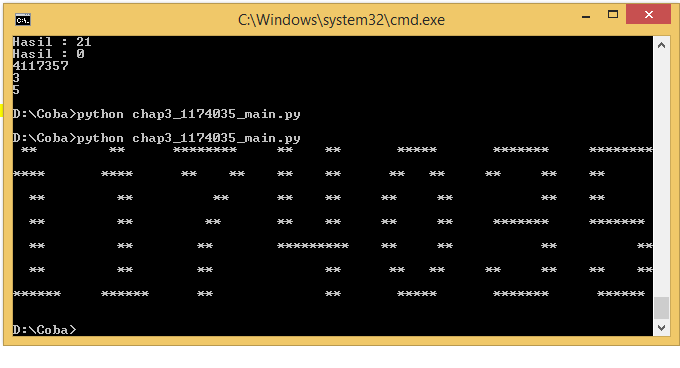
\includegraphics[height=7cm, width=10cm]{figures/chapter3/1174035_1.png}
        \caption{Screenshot No 1}
        \label{1174035_1}
	\end{figure}
	\item Membuat fungsi dengan inputan variabel NPM, dan lakukan perulangan untuk mengeluarkan print output sebanyak dua dijit belakang NPM. Contoh NPM : 1174035 maka akan ada output sebanyak 35 kali dengan tulisan 'Hallo, 1174035 apa kabar?' Kodingnya : 
	\lstinputlisting{src/chapter3/chap3_1174035_2.py}
	\begin{figure}[!htbp]
        \centering
        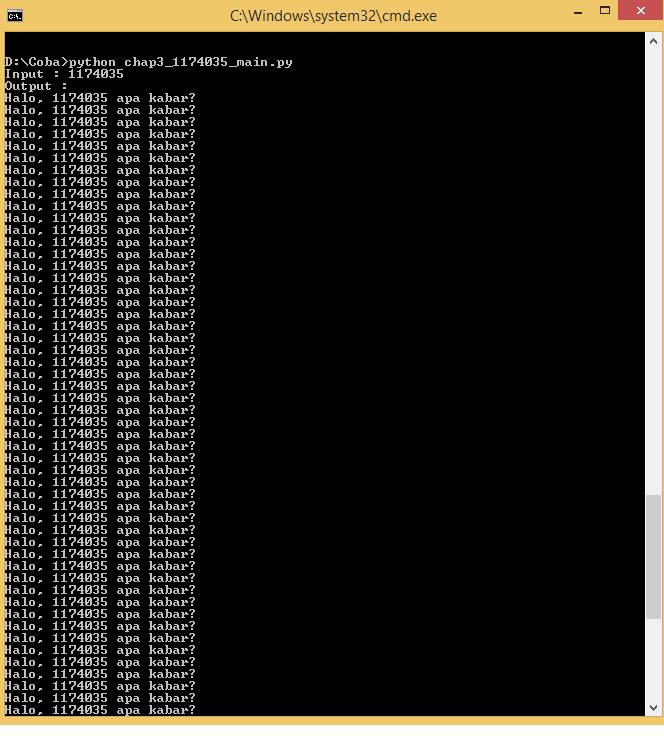
\includegraphics[height=7cm, width=10cm]{figures/chapter3/1174035_2.png}
        \caption{Screenshot No 2}
        \label{1174035_2}
	\end{figure}
	\item Membuat fungsi dengan inputan variabel NPM, dan melakukan print luaran output dengan perulangan berupa tiga karakter belakang dari NPM dijumlahkan. Lalu jumah perulangan tersebut adalah total dari tiga karakter belakang NPM dijumlahkan. Kodingnya : 
	\lstinputlisting{src/chapter3/chap3_1174035_3.py}
	\begin{figure}[!htbp]
        \centering
        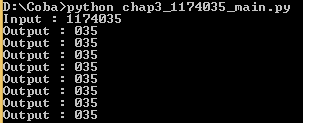
\includegraphics[height=7cm, width=10cm]{figures/chapter3/1174035_3.png}
        \caption{Screenshot No 3}
        \label{1174035_3}
	\end{figure}
	\item Membuat fungsi dengan inputan variabel NPM, dan melakukan print hello world dan digit ketiga dari belakang dari NPM. contoh : NPM : 0, Output : Halo, 0 apa kabar? .Kodingnya : 
	\lstinputlisting{src/chapter3/chap3_1174035_4.py}
	\begin{figure}[!htbp]
        \centering
        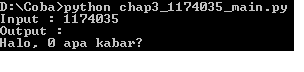
\includegraphics[height=3cm, width=8cm]{figures/chapter3/1174035_4.png}
        \caption{Screenshot No 4}
        \label{1174035_4}
	\end{figure}
	\item Membuat fungsi dengan inputan variabel NPM, dan menampilkan semua angka dari NPM tersebut secara berurutan kebawah. Kodingnya : 
	\lstinputlisting{src/chapter3/chap3_1174035_5.py}
	\begin{figure}[!htbp]
        \centering
        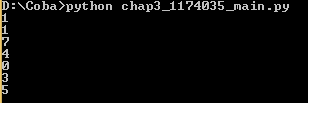
\includegraphics[height=5cm, width=10cm]{figures/chapter3/1174035_5.png}
        \caption{Screenshot No 5}
        \label{1174035_5}
	\end{figure}
	\item Membuat fungsi dengan inputan variabel NPM, didalamnya melakukan penjumlahan dari seluruh dijit NPM tersebut. menggunakan perulangan atau kondisi. Kodingnya : 
	\lstinputlisting{src/chapter3/chap3_1174035_6.py}
	\begin{figure}[!htbp]
        \centering
        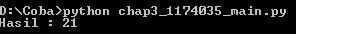
\includegraphics[height=5cm, width=10cm]{figures/chapter3/1174035_6.png}
        \caption{Screenshot No 6}
        \label{1174035_6}
	\end{figure}
	\item Membuat fungsi dengan inputan variabel NPM, didalamnya melakukan perkalian dari seluruh dijit NPM tersebut. menggunakan perulangan atau kondisi. Kodingnya : 
	\lstinputlisting{src/chapter3/chap3_1174035_7.py}
	\begin{figure}[!htbp]
        \centering
        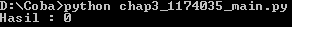
\includegraphics[height=4cm, width=10cm]{figures/chapter3/1174035_7.png}
        \caption{Screenshot No 7}
        \label{1174035_7}
	\end{figure}
	\item Membuat fungsi dengan inputan variabel NPM, lalu lakukan print seluruh angka genap dari setiap angka di NPM. Kodingnya : 
	\lstinputlisting{src/chapter3/chap3_1174035_8.py}
	\begin{figure}[!htbp]
        \centering
        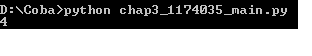
\includegraphics[height=4cm, width=10cm]{figures/chapter3/1174035_8.png}
        \caption{Screenshot No 8}
        \label{1174035_8}
	\end{figure}
	\item Membuat fungsi dengan inputan variabel NPM, lalu lakukan print seluruh angka ganjil dari setiap angka di NPM. Kodingnya : 
	\lstinputlisting{src/chapter3/chap3_1174035_9.py}
	\begin{figure}[!htbp]
        \centering
        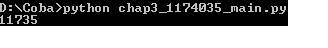
\includegraphics[height=4cm, width=10cm]{figures/chapter3/1174035_9.png}
        \caption{Screenshot No 9}
        \label{1174035_9}
	\end{figure}
	\item Membuat fungsi dengan inputan variabel NPM, lalu lakukan print seluruh angka prima dari setiap angka di NPM. Kodingnya : 
	\lstinputlisting{src/chapter3/chap3_1174035_10.py}
	\begin{figure}[!htbp]
        \centering
        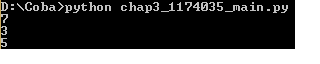
\includegraphics[height=5cm, width=10cm]{figures/chapter3/1174035_10.png}
        \caption{Screenshot No 10}
        \label{1174035_10}
	\end{figure}
	\item Membuat Satu File library bernama 3lib.py yang berisi semua fungsi - fungsi dari setiap nomor pada soal praktek. Kodingnya : 	
	\lstinputlisting{src/chapter3/chap3_1174035_3lib.py}
	\lstinputlisting[firstline=1, lastline=15]{src/chapter3/chap3_1174035_main.py}
	
	\begin{figure}[!htbp]
        \centering
        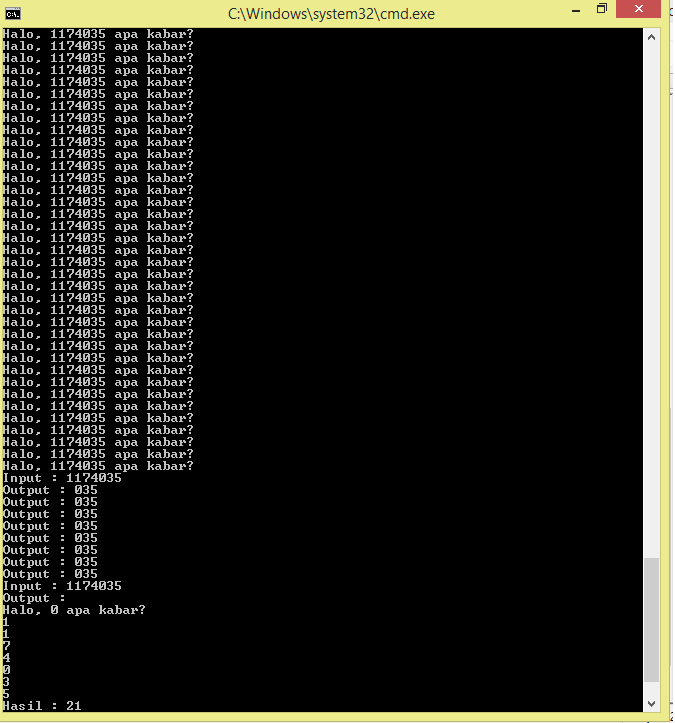
\includegraphics[height=10cm, width=8cm]{figures/chapter3/1174035_3lib.png}
        \caption{Screenshot No 11}
        \label{1174035_3lib}
	\end{figure}
	
	\item Membuat Satu File library bernama kelas3lib.py yang berisi kelas yang isinya semua fungsi - fungsi dari setiap nomor yang telah dimodifikasi untuk menyesuaikan dengan kelas. Kodingnya : 	
	\lstinputlisting{src/chapter3/chap3_1174035_kelas3lib.py}
	\lstinputlisting[firstline=16, lastline=29]{src/chapter3/chap3_1174035_main.py}
	
	\begin{figure}[!htbp]
        \centering
        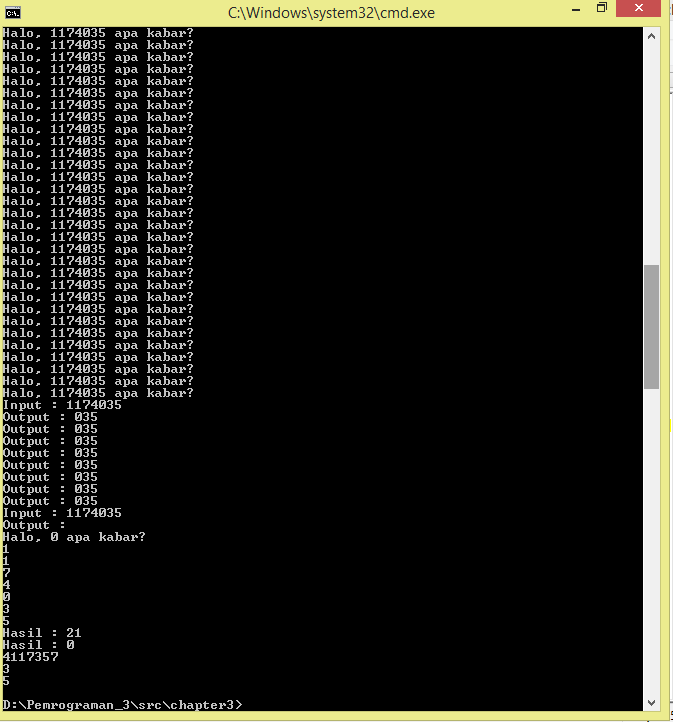
\includegraphics[height=10cm, width=8cm]{figures/chapter3/1174035_kelas3lib.png}
        \caption{Screenshot No 12}
        \label{1174035_kelas3lib}
	\end{figure}
	
	
\end{enumerate}

\subsubsection{Error}
\begin{enumerate}
	\item Tuliskan error yang terjadi saat mengerjakan section ini. Mendapat error yaitu salah konversi. Untuk menghandle error tersebut dapat menggunakan try catch :
	\lstinputlisting{src/chapter3/chap3_1174035_error.py}
	\lstinputlisting[firstline=32, lastline=36]{src/chapter3/chap3_1174035_main.py}
	\begin{figure}[!htbp]
        \centering
        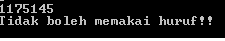
\includegraphics[height=3cm, width=8cm]{figures/chapter3/1174035_error.png}
        \caption{Screenshot No 13}
        \label{1174035_error}
	\end{figure}
	\item Plagiarisme
	\begin{figure}[!htbp]
        \centering
        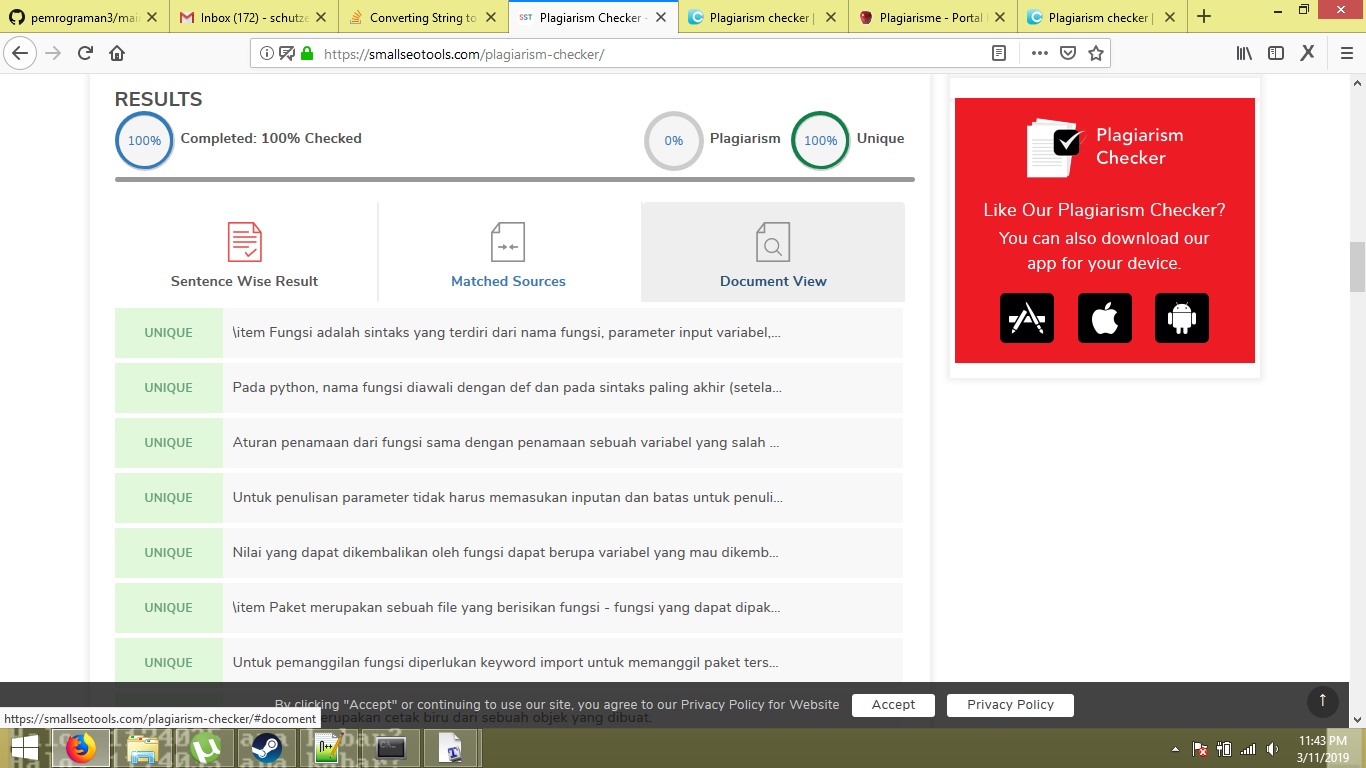
\includegraphics[height=7cm, width=9cm]{figures/chapter3/1174035_plagiarisme.png}
        \caption{Plagiarisme}
        \label{1174035_plagiarisme}
	\end{figure}
\end{enumerate}

\section{Rangga Putra Ramdhani}
\subsubsection{Pemahanan Teori}
\begin{enumerate}
    \item Apa itu fungsi, inputan fungsi dan kembalian fungsi dengan contoh kode program
    lainnya.
    Fungsi adalah bagian dari program yang dapat digunakan ulang.
    Berikut merupakan contoh fungsi dan cara pemanggilannya
    \lstinputlisting[firstline=124, lastline=127]{src/1174056_praktek.py}

    Fungsi dapat membaca parameter, parameter adalah nilai yang disediakan kepada fungsi, dimana nilai ini akan menentukan output yang akan dihasilkan fungsi.
    \lstinputlisting[firstline=129, lastline=132]{src/1174056_praktek.py}

    Statemen return digunakan untuk keluar dari fungsi. Kita juga dapat menspesifikasikan nilai kembalian.
    \lstinputlisting[firstline=134, lastline=141]{src/1174056_praktek.py}

    \item Apa itu paket dan cara pemanggilan paket atau library dengan contoh kode
    program lainnya.
    Untuk memudahkan dalam pemanggilan fungsi yang di butuhkan, agar dapat dipanggil berulang.
    Cara pemanggilannya
    \lstinputlisting[firstline=143, lastline=144]{src/1174056_praktek.py}

    \item Jelaskan Apa itu kelas, apa itu objek, apa itu atribut, apa itu method dan
    contoh kode program lainnya masing-masing.
    kelas merupakan sebuah blueprint yang mepresentasikan objek.
    objek adalah hasil cetakan dadri sebuah kelas.
    method adalah suatu upaya yang digunakan oleh object.
    \lstinputlisting[firstline=146, lastline=168]{src/1174056_praktek.py}

    \item Jelaskan cara pemanggikan library kelas dari instansiasi dan pemakaiannya den-
    gan contoh program lainnya.
    Cara Pemanggilanya 
    \begin{itemize}
        \item pertama import terlebih dahulu filenya.
        \item kemudian buat variabel untuk menampung datanya
        \item setelah itu panggil nama classnya dan panggil methodnya
        \item Gunakan perintah print untuk menampilkan hasilnya

    \end{itemize}
    \lstinputlisting[firstline=170, lastline=175]{src/1174056_praktek.py}

    \item Jelaskan dengan contoh pemakaian paket dengan perintah from kalkulator im-
    port Penambahan disertai dengan contoh kode lainnya.
    Penggunaan paket from namafile import, itu berfungsi untuk memanggil file dan fungsinya
    \lstinputlisting[firstline=143, lastline=144]{src/1174056_praktek.py}

    \item Jelaskan dengan contoh kodenya, pemakaian paket fungsi apabila le library
    ada di dalam folder.
    Pemakaian paket adalah perkumpulan fungsi-fungsi. contoh kodenya adalah sebagai berikut :

    \item Jelaskan dengan contoh kodenya, pemakaian paket kelas apabila le library ada
    di dalam folder.
    \lstinputlisting[firstline=184, lastline=184]{src/1174056_praktek.py}

\end{enumerate}
\subsubsection{Ketrampilan Pemrograman}
\begin{enumerate}
    \item Buatlah fungsi dengan inputan variabel NPM, dan melakukan print luaran huruf
    yang dirangkai dari tanda bintang, pagar atau plus dari NPM kita. Tanda
    bintang untuk NPM mod 3=0, tanda pagar untuk NPM mod 3 =1, tanda plus
    untuk NPM mod3=2.
    \lstinputlisting[firstline=184, lastline=234]{src/1174056_praktek.py}

    \item Buatlah fungsi dengan inputan variabel berupa NPM. kemudian dengan meng-
    gunakan perulangan mengeluarkan print output sebanyak dua dijit belakang
    NPM.
    \lstinputlisting[firstline=237, lastline=243]{src/1174056_praktek.py}

    \item Buatlah fungsi dengan dengan input variabel string bernama NPM dan beri
    luaran output dengan perulangan berupa tiga karakter belakang dari NPM se-
    banyak penjumlahan tiga dijit tersebut.
    \lstinputlisting[firstline=245, lastline=255]{src/1174056_praktek.py}

    \item Buatlah fungsi hello word dengan input variabel string bernama NPM dan
    beri luaran output berupa digit ketiga dari belakang dari variabel NPM meng-
    gunakan akses langsung manipulasi string pada baris ketiga dari variabel NPM.
    \lstinputlisting[firstline=257, lastline=263]{src/1174056_praktek.py}

    \item buat fungsi program dengan input variabel NPM dan melakukan print nomor npm satu persatu kebawah.
    \lstinputlisting[firstline=265, lastline=269]{src/1174056_praktek.py}

    \item Buatlah fungsi dengan inputan variabel NPM, didalamnya melakukan penjum-
    lahan dari seluruh dijit NPM tersebut, wajib menggunakan perulangan dan
    atau kondisi.
    \lstinputlisting[firstline=272, lastline=279]{src/1174056_praktek.py}

    \item Buatlah fungsi dengan inputan variabel NPM, didalamnya melakukan melakukan
    perkalian dari seluruh dijit NPM tersebut, wajib menggunakan perulangan dan
    atau kondisi.
    \lstinputlisting[firstline=281, lastline=288]{src/1174056_praktek.py}

    \item Buatlah fungsi dengan inputan variabel NPM, Lakukan print NPM anda tapi
    hanya dijit genap saja. wajib menggunakan perulangan dan atau kondisi.
    \lstinputlisting[firstline=290, lastline=296]{src/1174056_praktek.py}

    \item Buatlah fungsi dengan inputan variabel NPM, Lakukan print NPM anda tapi
    hanya dijit ganjil saja. wajib menggunakan perulangan dan atau kondisi.
    \lstinputlisting[firstline=298, lastline=304]{src/1174056_praktek.py}

    \item Buatlah fungsi dengan inputan variabel NPM, Lakukan print NPM anda tapi
    hanya dijit yang termasuk bilangan prima saja. wajib menggunakan perulangan
    dan atau kondisi.
    \lstinputlisting[firstline=306, lastline=320]{src/1174056_praktek.py}

    \item Buatlah satu library yang berisi fungsi-fungsi dari nomor diatas dengan nama
    le rangga.py dan berikan contoh cara pemanggilannya pada le main.py.
    \lstinputlisting[firstline=7, lastline=7]{src/mainn.py}

    \item Buatlah satu library class dengan nama le kelas3lib.py yang merupakan mod-
    ikasi dari fungsi-fungsi nomor diatas dan berikan contoh cara pemanggilannya
    pada le mainn.py.
    \lstinputlisting[firstline=8, lastline=9]{src/mainn.py}
    
\end{enumerate}
\subsubsection{Ketrampilan Penanganan Error}
Error yang di dapat dari mengerjakan tugas ini adalah type error, cara menaggulaginya dengan cara mengecheck kembali codingannya
kemudian run kembali aplikasinya
berikut contoh Penggunaan fungsi try dan exception
\lstinputlisting[firstline=177, lastline=182]{src/1174056_praktek.py}


\section{Faisal Najib Abdullah}
\subsection{Pemahanan Teori}
\begin{enumerate}
    \item Apa itu fungsi, inputan fungsi dan kembalian fungsi dengan contoh kode program
    lainnya.
    Fungsi adalah bagian dari program yang dapat digunakan ulang.
    Berikut merupakan contoh fungsi dan cara pemanggilannya
    \lstinputlisting{src/chapter3/1174042_1,1.py}

    Fungsi dapat membaca parameter, parameter adalah nilai yang disediakan kepada fungsi, dimana nilai ini akan menentukan output yang akan dihasilkan fungsi.
    \lstinputlisting{src/chapter3/1174042_1,1,1.py}

    Statemen return digunakan untuk keluar dari fungsi. Kita juga dapat menspesifikasikan nilai kembalian.
    \lstinputlisting{src/chapter3/1174042_1,1,2.py}

    \item Apa itu paket dan cara pemanggilan paket atau library dengan contoh kode
    program lainnya.
    Untuk memudahkan dalam pemanggilan fungsi yang di butuhkan, agar dapat dipanggil berulang.
    Cara pemanggilannya
    \lstinputlisting{src/chapter3/1174042_1,2.py}

    \item Jelaskan Apa itu kelas, apa itu objek, apa itu atribut, apa itu method dan
    contoh kode program lainnya masing-masing.
    kelas merupakan sebuah blueprint yang mepresentasikan objek.
    objek adalah hasil cetakan dadri sebuah kelas.
    method adalah suatu upaya yang digunakan oleh object.
    \lstinputlisting{src/chapter3/1174042_1,3.py}

    \item Jelaskan cara pemanggikan library kelas dari instansiasi dan pemakaiannya den-
    gan contoh program lainnya.
    Cara Pemanggilanya 
    \begin{itemize}
        \item pertama import terlebih dahulu filenya.
        \item kemudian buat variabel untuk menampung datanya
        \item setelah itu panggil nama classnya dan panggil methodnya
        \item Gunakan perintah print untuk menampilkan hasilnya

    \end{itemize}
    \lstinputlisting{src/chapter3/1174042_1,4.py}

    \item Jelaskan dengan contoh pemakaian paket dengan perintah from kalkulator im-
    port Penambahan disertai dengan contoh kode lainnya.
    Penggunaan paket from namafile import, itu berfungsi untuk memanggil file dan fungsinya
    \lstinputlisting{src/chapter3/1174042_1,2.py}

    \item Jelaskan dengan contoh kodenya, pemakaian paket fungsi apabila file library
    ada di dalam folder.
    Pemakaian paket adalah perkumpulan fungsi-fungsi. contoh kodenya adalah sebagai berikut :
	\lstinputlisting{src/chapter3/1174042_1,6.py}

    \item Jelaskan dengan contoh kodenya, pemakaian paket kelas apabila file library ada
    di dalam folder.
    \lstinputlisting{src/chapter3/1174042_1,6.py}
\end{enumerate}
\subsection{Ketrampilan Pemrograman}
\begin{enumerate}
    \item Buatlah fungsi dengan inputan variabel NPM, dan melakukan print luaran huruf
    yang dirangkai dari tanda bintang, pagar atau plus dari NPM kita. Tanda
    bintang untuk NPM mod 3=0, tanda pagar untuk NPM mod 3 =1, tanda plus
    untuk NPM mod3=2.
    \lstinputlisting{src/chapter3/1174042_2,1.py}

    \item Buatlah fungsi dengan inputan variabel berupa NPM. kemudian dengan meng-
    gunakan perulangan mengeluarkan print output sebanyak dua dijit belakang
    NPM.
    \lstinputlisting{src/chapter3/1174042_2,2.py}

    \item Buatlah fungsi dengan dengan input variabel string bernama NPM dan beri
    luaran output dengan perulangan berupa tiga karakter belakang dari NPM se-
    banyak penjumlahan tiga dijit tersebut.
    \lstinputlisting{src/chapter3/1174042_2,3.py}

    \item Buatlah fungsi hello word dengan input variabel string bernama NPM dan
    beri luaran output berupa digit ketiga dari belakang dari variabel NPM meng-
    gunakan akses langsung manipulasi string pada baris ketiga dari variabel NPM.
    \lstinputlisting{src/chapter3/1174042_2,4.py}

    \item buat fungsi program dengan input variabel NPM dan melakukan print nomor npm satu persatu kebawah.
    \lstinputlisting{src/chapter3/1174042_2,5.py}

    \item Buatlah fungsi dengan inputan variabel NPM, didalamnya melakukan penjum-
    lahan dari seluruh dijit NPM tersebut, wajib menggunakan perulangan dan
    atau kondisi.
    \lstinputlisting{src/chapter3/1174042_2,6.py}

    \item Buatlah fungsi dengan inputan variabel NPM, didalamnya melakukan melakukan
    perkalian dari seluruh dijit NPM tersebut, wajib menggunakan perulangan dan
    atau kondisi.
    \lstinputlisting{src/chapter3/1174042_2,7.py}

    \item Buatlah fungsi dengan inputan variabel NPM, Lakukan print NPM anda tapi
    hanya dijit genap saja. wajib menggunakan perulangan dan atau kondisi.
    \lstinputlisting{src/chapter3/1174042_2,8.py}

    \item Buatlah fungsi dengan inputan variabel NPM, Lakukan print NPM anda tapi
    hanya dijit ganjil saja. wajib menggunakan perulangan dan atau kondisi.
    \lstinputlisting{src/chapter3/1174042_2,9.py}

    \item Buatlah fungsi dengan inputan variabel NPM, Lakukan print NPM anda tapi
    hanya dijit yang termasuk bilangan prima saja. wajib menggunakan perulangan
    dan atau kondisi.
    \lstinputlisting{src/chapter3/1174042_2,10.py}

    \item Buatlah satu library yang berisi fungsi-fungsi dari nomor diatas dengan nama
    file 3lib.py dan berikan contoh cara pemanggilannya pada file main.py.
    \lstinputlisting{src/chapter3/1174042_main.py}

    \item Buatlah satu library class dengan nama file kelas3lib.py yang merupakan mod-
    ifikasi dari fungsi-fungsi nomor diatas dan berikan contoh cara pemanggilannya
    pada file main.py.
    \lstinputlisting{src/chapter3/1174042_main.py}
    
\end{enumerate}
\subsection{Ketrampilan Penanganan Error}
Error yang di dapat dari mengerjakan tugas ini adalah type error, cara menaggulaginya dengan cara mengecheck kembali codingannya
kemudian run kembali aplikasinya
berikut contoh Penggunaan fungsi try dan exception
\lstinputlisting{src/chapter3/1174042_2err.py}
